
%%%%%%%%%%%%%%%%%%%%%%%%%%%%%%%%%%%%%%%%%%%%%%%%%%%%%%%%%%%%%%%%%%%%%%%%%%%%%%%%%%%%%%%%%%%%%%%%%%%%%%%
% Parallelization of Homology Search
%%%%%%%%%%%%%%%%%%%%%%%%%%%%%%%%%%%%%%%%%%%%%%%%%%%%%%%%%%%%%%%%%%%%%%%%%%%%%%%%%%%%%%%%%%%%%%%%%%%%%%%

\fancychapter{Parallelization of Homology Search}

This chapter will review the most promising and well-studied techniques for parallelization of Homology Search, both of classical Alignment algorithms and Profile HMMs algorithms. The first section will deal with the parallelization of Alignment algorithms, and the later section will focus on the parallelization of Profile HMMs, which employ the same strategies, as it will be explained.

Parallelization approaches can be divided in Intra-task parallelism, wherein each alignment task is itself parallelized; and Inter-task parallelism, which consists of running multiple tasks (in this case, multiple alignments) in parallel.

\section{Parallelization of Alignment Algorithms}
\label{Parallelization of Alignment Algorithms}

\subsection{Instruction-level Parallelism and Code Optimization}

Scalar instruction-level parallelism in sequence alignment has been described by various authors such as Alpern \cite{alpern}, Szalkowski in SWPS3 (\cite {swps3}), Farrar \cite{farrarcell}, Rudnicki \cite{rudnicki2009cell}, \cite{rognes2011} and others. It is usually achieved by carefully re-arranging the instructions, normally done by the compiler or processor itself, in order to exploit the available processing pipelines on modern superscalar architectures. Special care must be taken on the implementation of very tight loops to allow the processor and compiler to better re-organize and parallelize the sequential code. The main concern is the removal of data dependencies and divergent execution paths (conditional branches).

Moreover, modern processors also employ many speculative optimization techniques, such as out-of-order execution and branch prediction. All these depend on the parallelization potential of sequential code, and as such, any un-parallelizable code section leads to a drastic performance cut. In particular, branch mis-predictions cause the whole pipeline to be flushed out, and all instructions already speculatively executed are discarded.

Another concern is the cache use: data locality is of the utmost importance, as well as the cache size itself, which determines how much of the inner variables and data can fit into cache. The cache size available, and the conscious and explicit optimization for such size, has a dramatic influence on the overall performance. A program with optimal cache utilization may come near a 100\% cache hit rate on the innermost loops that can fit into cache, and hence achieve an enormous speedup on the global runtime.

Many strategies have been described on this level to carefully hand-tune the most critical assembly code, such as:

- loop unrolling of the innermost loop \cite{alpern}, \cite{rognes2011}, so that it processes two or more iterations sequentially at a time. This reduces the number of inner branches, and hints the processor to parallelize the two iterations on the available concurrent execution pipelines;

- tiling of loops (strip-mining) to improve cache reuse \cite{alpern}. This technique consists of transforming a single loop into two nested loops, thus reducing the inner-loop length, to ensure that the inner-loop data stays in cache;

- reduce and remove any possible conditional branch, especially in the inner loops. In many cases, they can be moved out to the outer loops, initialization sections, or external same-level loops. This comes at the cost of some repeated or redundant work, but it is a small price to pay.
	



%%%%%%%%%%%%%%%%%%%%%%%%%%%%%%%%%%%%%%%%%%%%%%%%%%%%%%%%%%%%%%%%%%%%%%%
%%%%%%%%%%%%%%%%%%%%%%%%%%%%%%%%%%%%%%%%%%%%%%%%%%%%%%%%%%%%%%%%%%%%%%%

\subsection{Fine-grained Parallelism using SIMD units}

Fine-grained parallelism is implemented on the lowest instruction level. Besides the mechanisms described in the previous section, it can also be achieved through vector (SIMD) processing.

By now, SIMD extensions have already a reasonable long history of use and success. They implement a Single-Instruction/Multiple-Data parallel model on scalar CPUs, through the use of specialized vector processing units. Several of these instruction set extensions have enjoyed a considerable success, such as MMX/SSE on Intel and AMD's 3Dnow. One of most widely available is the SSE extensions on Intel processors. Each SSE register has 128-bits, capable of storing four 32-bit integers (rarely needed for alignment), eight 16-bit short integers (these can be used for alignments that reach high scores - such as very long sequences, very similar sequences, or very high base scores/penalties), or sixteen 8-bit bytes (the common case, allowing scores up to 255). Each stored element/value defines a single sequential 'execution channel'.

The first use of SIMD extensions for alignment tasks in general-purpose processors was employed by Alpern \cite{alpern} in 1995, using 64bit registers to simulate SIMD vectors. Others followed quickly,  using different parallelization strategies and decomposition patterns, on an increasing variety of different architectures (VAX mini-computers, Intel Pentiums, Cell BE, etc).


\subsubsection{Decomposition Patterns in Intra-task Parallelism}
\label{Decomposition Patterns in Intra-task Parallelism}

When employing SIMD vector processing, using each matrix cell computation as a \emph{primitive task}, the direction in which the cells are processed is of paramount importance. It determines how dependencies are parallelized, how many can be parallelized, and how costly it is to resolve the serial (non-parallelized) dependencies. When using SIMD units, the greatest obstacle is the dependencies within each SIMD vector (i.e. between the N parallel elements in the same N-channel SIMD unit vector). It is the most decisive factor in the overall performance.

Three main parallel decomposition patterns have been studied over the last decades to tackle the difficult problem of parallelizing data dependencies in intra-task parallelism: 

\myparagraph{Decomposition in a Diagonal Pattern}
\label{section-wozniak}

The most natural vectorial pattern to process the alignment matrix is by following the direction of the data dependencies, which is a diagonal direction \autoref{pattern-diagonal}. Processing each anti-diagonal in parallel is therefore a good method that was first proposed by Wozniak \cite{wozniak} in 1997 and often adopted ever since. One major advantage of this pattern is that it has no conditional branches in the inner loop. Still, it has one serious drawback: the heavy cost of the basic operations, required to diagonally access and process the matrix. Moreover, the diagonal pattern restricts the applicability of some precious optimizations, such as the the one proposed by Green in SWAT (see \sref{SWAT optimization}).

\myparagraph{Decomposition in a Vertical (or Horizontal) Continuous Pattern}
\label{section-rognes1}
		
Processing each column (or line) of the matrix in parallel is the other natural approach, perhaps the simplest and most intuitive \autoref{pattern-continuous}. This pattern has also been thoroughly employed, with some very optimized and efficient implementations, starting with Rognes \cite{rognes2000} in 2000 . The main problem of this strategy is the vertical (or horizontal, when parallelizing by lines) dependencies, which cannot be parallelized - they must be resolved sequentially, in a scalar way, amidst the SSE code, which is very inefficient.


\myparagraph{Decomposition in a Vertical (or Horizontal) Striped Pattern}
\label{section-farrar}

Building on Rognes solution, Farrar \cite{farrar} in 2007 devised a striped pattern decomposition to tackle the problem of vertical dependencies \autoref{pattern-striped}. Through the use of a striped pattern, beside the parallelization of horizontal and diagonal dependencies, it is also  possible to parallelize the vertical dependencies: each element j of the $i$-th segment will influence the same element j of the $(i+1)$-th segment. The biggest remaining problem is the dependencies across 'segment sections' (continuous sections) - in Farrar's algorithm, these are processed later, in a second inner loop (\emph{Lazy-F loop}), and following a SWAT-like optimization (i.e. the F values may only have any effect if they are higher than $W_1$). Despite the striped decomposition's better results, it is also less flexible and less prone to extension and customization (for instance, to run banded alignments). Moreover, for very short sequences, the striped pattern has an overhead (mostly from the Lazy-F loop) that is not easily amortized.

\begin{figure}[htb!]
\centering
\mbox{
	\subfigure[Decomposition in anti-diagonals. The lower, upper, and right sides are padded.]{
		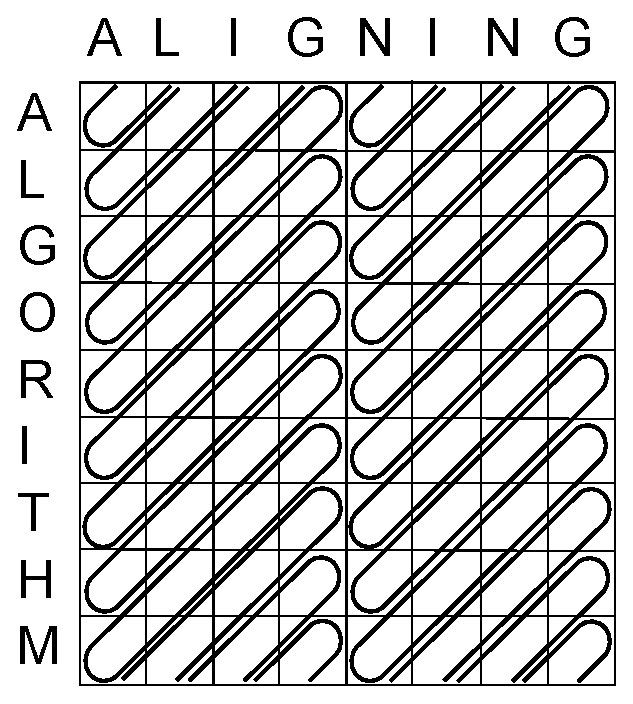
\includegraphics[scale=0.45]{img-par/pattern-diagonal.eps}
		\label{pattern-diagonal}
	}
	\quad
	\subfigure[Decomposition in continous lines. The lower side (last segment per column) is padded.]{
		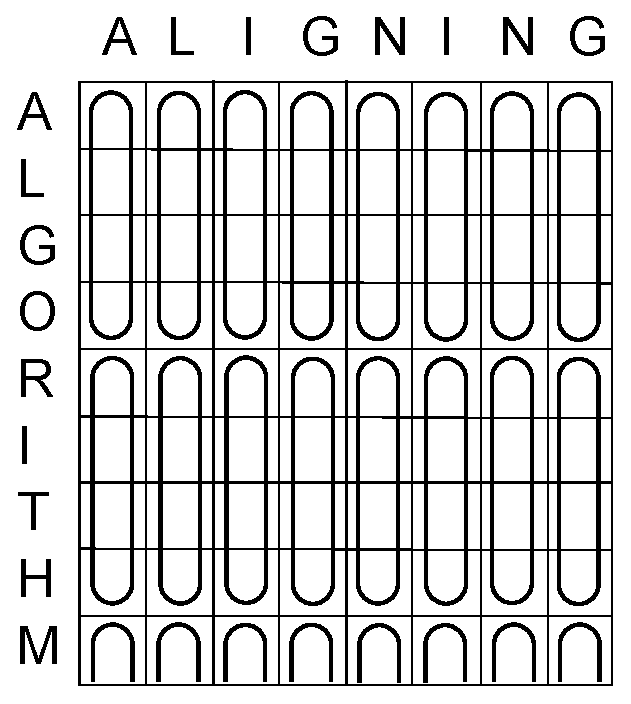
\includegraphics[scale=0.45]{img-par/pattern-continuous.eps}
		\label{pattern-continuous}
	}
	\quad
	\subfigure[Decomposition in striped lines. Each segment is padded.]{
		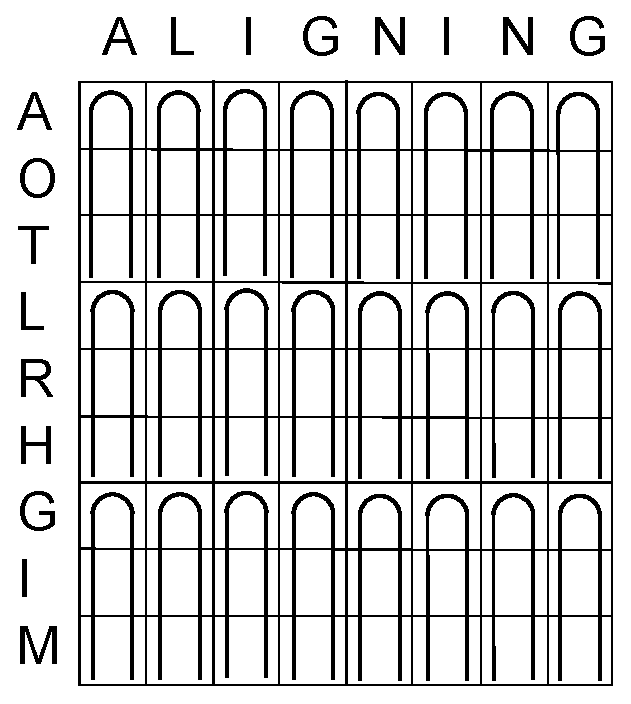
\includegraphics[scale=0.45]{img-par/pattern-striped.eps}
		\label{pattern-striped}
	}
}
\caption{Decomposition patterns for intra-task parallelism}
\end{figure}




%%%%%%%%%%%%%%%%%%%%%%%%%%%%%%%%%%%%%%%%%%%%%%%%%%%%%%%%%%%%%%%%%%%%%%%
%%%%%%%%%%%%%%%%%%%%%%%%%%%%%%%%%%%%%%%%%%%%%%%%%%%%%%%%%%%%%%%%%%%%%%%
		
\subsubsection{Main Problems of SIMD Intra-task parallelism}
		
There are several  issues afflicting SIMD algorithms, the most serious being:

\myparagraph{Limited Range of the parallel SIMD elements}

To maximize the algorithm's throughput, it is naturally desired to process as many elements in parallel as possible. This leads to fields of 8bits (1byte) for each element, which can have a maximum range of merely 255 (assuming only positive scores and penalties, or convert them to be such). For short sequences and reasonable typical scoring values, this is usually enough, but not always. Very similar sequences can easily overflow the 255-range, which invalidates the final score obtained, and forces alignment to be repeated with a higher range.
			
\myparagraph{Scoring matrices}

It is costly to access scoring matrices. Each access requires two indirections, one to find the sequence residue, and the other when the residue is used to access the matrix of scores. When using SIMD instructions, this problem increases tenfold - each vector element requires a different score, but those are scattered over the matrix (which is indexed by residue value, both in lines and columns).
	
\myparagraph{Divergent execution paths}

Divergent execution paths are  introduced by conditional branches in the inner loops, which in practice turn the theoretical parallel code into scalar code. Furthermore, these hamper the processor's pipeline and branch prediction. One example is the required branches when processing the vertical dependencies within a SIMD vector.

\myparagraph {Scalar sequential code}

Some inherently scalar sequential code cannot simply be parallelized. For instance, the vertical dependencies cannot be fully parallelized, as well as the initialization scalar values. These singular cases require manipulation of the internal SSE elements with cumbersome vector instructions, such as shifts, packs and shuffles, to simulate simple scalar operations.

\myparagraph {Cache Storage}

A fundamental issue is the cache availability to store the arrays of SSE vectors used in the innermost loops: one E array, one of two H array(s), the F value, several auxiliary variables and constant values (variable names taken from Gotoh's equations, see \sref{Gotoh algorithm}). A lazy tuning of the inner loops data to the cache storage size may considerably impair the overall system performance.

\myparagraph {Banded Alignment}

Banded alignment brings new challenges to vectorial parallelism. Farrar's striped pattern works very well for long runs, but the Lazy-F loop overhead becomes a problem in very small runs (a band width of 30 bases can fit entirely in two SSE vectors). Another problem is the frequent inner-loop re-initializations. 
%TODO MAIS COISAS
Regarding the query profiles, their loading onto the SSE registers also induces an additional problem, since the memory becomes unaligned when processing each new column starting one cell later.
	
	
\subsubsection{Improvements for SIMD Algorithms}

To solve these main problems and improve the SIMD implementations, a few clever optimizations have been proposed:

\myparagraph{Unsigned and Saturated Arithmetic}

In order to increase the SIMD elements available range, unsigned arithmetic can be used, thus doubling the maximum range.

To deal with negative values, all scores and matrix cells are biased by a fixed small amount that guarantees no negative scores. Saturated arithmetic is then used to prevent values from dropping below 0 (and underflowing), as well as capping the values at the maximal value, preventing overflows. The minimum operation of the \ac{SW} algorithm is also spared, being replaced by the implicit sature-to-zero operation. Underflows correspond to the maximum operation with 0, and are part of the algorithm. Overflows, on the contrary, are an error introduced by the limited range used, and are used as a sign that the whole procedure needs to be repeated with a higher range. As such, the test for the correctness of the alignment needs only to be done in the end, and it is simply '\emph{final score \textgreater MaxValue - Bias}'.

There are cases however, when this mechanism cannot be used, as necessary architectural support is lacking. For instance, SSE only supports  signed arithmetic for short values (16bit). To overcome this obstacle, some emulations of unsigned saturated arithmetic were devised. Farrar biased all values with -32k (the short min value), and then used saturated signed arithmetic to solve the problem. Rognes \cite{rognes2011} in 2011 used a similar approach in the 7bit range, with both saturated arithmetic and unsaturated maximum, to avoid the Add instruction needed to unbias the scores.
		
For architectures without any support for saturation, Farrar \cite{farrarcell} proposed a different biasing procedure. The idea is to add a small bias to every value, maximize each computed value with this bias (preventing it from dropping below 0), and testing for overflow with '\emph{value \textgreater MaxValue - Bias}'.

\myparagraph{Query-specific scoring profile}
\label{scoring-profile}

Packing each element at a time into the required SSE vector would be a considerable bottleneck. To avoid this, the substitution scores must be stored sequentially (or striped in Farrar's version) in memory, according to the respective sequence elements, so that a single load instruction can fetch the whole SSE vector from the substitution matrix in memory onto a register. The result is a new scoring matrix adapted to the query sequence, called a query-specific scoring profile.

The storage required for such a profile can also easily grow out of hand, especially for very large queries. This is a serious problem in computers with very small on-chip memory (GPUs and Cell's synergistic processors, for instance). The mechanism described in the next paragraph attempts to minimize this problem. 
		
\myparagraph{Compacting and expanding scoring profiles}

A possible method to compact the scoring profile was proposed in \cite{swps3}. The idea is to use the minimum required memory to keep the substitution scores (normally only 1byte per value), and expand them to larger sizes using SSE's unpack instruction, when executing with 16bit of higher elements' ranges. The sequences themselves can also be compacted with 2bits per base. 

%\myparagraph{Scaled Offset Map}
%A recent original ideia has been presented \cite{scaledmap} 
%A possible strategy to support much larger scores, while still using the same limited 8bit elements, is the usage of a scaled offset map. It consists of a checker-block divided matrix with offset factors to represent higher-ranged scores. Each square block of the \ac{DP} matrix keeps an offset scale coefficient that gives a constant offset for the scores of the whole block when multiplied by a constant offset base value. This offset scale is determined at the boundaries between blocks, such that no possible variation within the same block can surpass the constant offset base.

%This mechanism introduces an overhead in the blocks' boundaries, as well as more storage needed to keep the offsets, so it is only useful when most alignments run in the limited range with a small but still considerable fraction needing higher ranges.
% When most alignments need the 16bit range, it is also not practical to use this, since it entails the overhead... ERRADO o overhead  e' constante independente das scores
	
\myparagraph{Optimizations of the Lazy-F loop}

Some optimizations have been studied for Farrar's Lazy-F loop \cite{swps3} \cite{farrarcell}, and achieved good results. One of the improvements consists mainly on relaxing the loop termination condition, since the original Lazy-F loop has in the worst case N (the complete column length) iterations. The other idea is moving some of the conditionals to a more external (and hence, less executed) position.

%estudar e expandir isto



\subsubsection{SIMD Implementation of Global Alignment}

As it has been described in \sref{Smith-Waterman algorithm for Local Alignment}, global alignment (in particular the \ac{NW} algorithm) differs from local alignment (\ac{SW}) in that the alignment must cover the whole sequences instead of just partial, positive-scoring, subsequences. Global alignment can be regarded as subproblem of local alignment when the start and end point of the alignment are fixed. The \ac{NW} algorithm, being a somehow reduced form of the \ac{SW} algorithm, is also and more efficient and simpler to implement. The main differences in the implementation are the following:
	
- No need to keep the best score found. The resulting alignment score is always the score of the last (rightmost) cell. A maximum operation in the inner loops is thus spared
	
- No need to use a zero lower bound - the maximization with 0 is also avoided.

- No alignment re-runs due to overflowing: Considering that, increasing scores can be used instead of decreasing, the values' range will always be positive; hence there are no underflows and lower-bound saturation is not needed. Higher-bound saturation is still needed to avoid wrap-around's. However, the overflown cells no longer constitute a problem since they have an extremely poor score (the higher the cell value, the worse it is). They are merely an innocuous side-effect of the procedure. In principle, they will never be chosen by the recursion's rule, and thus can be safely ignored. Actually, this may not be always the case, if the used arithmetic range is very ill-adjusted to the sequences. For correctly parametrized alignments, this technique can generally be safely used.
	
- Given that the start and endpoints of the alignment are known, some tuning of the algorithm can be done (for instance, heuristic filters and metrics).	%EXPANDIR MAIS ISTO
	
% TODO => Varios optimizacoes possiveis das implementacoes SW estudadas, qd passadas a globais




%%%%%%%%%%%%%%%%%%%%%%%%%%%%%%%%%%%%%%%%%%%%%%%%%%%%%%%%%%%%%%%%%%%%%%%
%%%%%%%%%%%%%%%%%%%%%%%%%%%%%%%%%%%%%%%%%%%%%%%%%%%%%%%%%%%%%%%%%%%%%%%

\subsection{Intra-task Parallelism on Multiple Cores}

Middle-level parallelism is achieved by dividing the \ac{DP} matrix in 'chunks' that can then be processed in parallel by the different cores on a single machine. This can also be extended to a grid of compurers, with each node processing a chunk, when the sequences are quite large. Several recent applications have been developed using this paradigm (\cite{liao2004parallel}, \cite{meng2005exploiting}, \cite{framework2010parallel}, \cite{hosny}).

This middle-level approach is much easier to implement than the fine-grained SSE: this one follows a simple MIMD model, in which each single processing datapath can diverge without any penalty, contrary to the SIMD model of vector processing that binds all the datapaths together. 

The first issue to consider in this level is the order in which the chunks are processed. Which ones can be processed in parallel? How many at the same time? The strategy that seems to work best is by parallelizing along each anti-diagonal (similar to Wozniak's fine-grained pattern \cite{wozniak}), which is the natural direction of the algorithm's dependencies. This leads to a so-called "tiled-chunk pattern" (each diagonal of chunks being seen as a tile). Authors in \cite{boukerche2007parallel}, \cite{zalign} and \cite{hosny} use this pattern. The order in which the chunks are processed is not very strict: they can advance vertically or horizontally. The only restriction is that each chunk above and to the left must be processed before.

To minimize the communication cost of exchanging values between cores, each one should process a chunk as large as possible in each iteration. The best layout is to use a single chunk per process per level (communication round). Each chunk should have roughly close to $\frac{N}{P}$ columns (or rows vice versa, $N$ columns, $P$ processors) , so that the computational work is balanced among all cores.  As for rows, each chunk can have any number of them. In particular they can have only one row, allowing for a finer-grain parallel decomposition \cite{boukerche2007parallel} (especially useful when the communication cost is low, such as when using shared symmetric memory multiprocessors). Note that the score matrix is an abstract concept: in practice the Gotoh linear-space algorithm is always employed, and only a couple of arrays are needed.

When using a granularity of one for columns and rows (1 cell for each chunk), each diagonal only depends on the past two diagonals (the previous one for vertical and horizontal dependencies, and the other for the diagonal dependencies). When using larger chunks, the data requirements are much better: each diagonal front needs only a 'stair-shaped' previous diagonal chunk-frontier (with $M+N$ cells, $M$ columns, $N$ rows). Since each diagonal has $a \times N$ cells (arbitrary granularity, $a$), the needed data-to-computation ratio is quite good. On the other hand, the higher the granularity is, the slower becomes the initial start-up time when some cores are idle waiting for available chunks.

Several alternative algorithmic strategies have been proposed to decompose the matrix between workers (such as ParAlign \cite{paralign} and GCM-BSP \cite{parbcp}). These use exploitable properties of the algorithms to split the computing space among parallel nodes, and later merge the results, usually with some restriction or accuracy loss. Most of these algorithms also only work for global alignment, since the 'restarting' step of local alignment is much more unpredictable.

% (EXPANDIR ESTAS TECNICAS)


%%%%%%%%%%%%%%%%%%%%%%%%%%%%%%%%%%%%%%%%%%%%%%%%%%%%%%%%%%%%%%%%%%%%%%%
%%%%%%%%%%%%%%%%%%%%%%%%%%%%%%%%%%%%%%%%%%%%%%%%%%%%%%%%%%%%%%%%%%%%%%%

\subsection{Inter-task Parallelism}
\label{Inter-task Parallelism}

Besides parallelizing a single alignment task, it is also possible to process multiple alignment matrices in parallel too (a single cell, or chunk, of each matrix at a time). This alternative method has also been much studied in the last decade.


\subsubsection{SIMD extensions}
\label{Rognes-section}

Instead of using a SIMD vector to process multiple cells of the same alignment matrix, we could feed a single cell from multiple matrices to each one of the independent parallel channels. This approach was first proposed by Alpern \cite{alpern} in 1995, and later extended and improved by Rognes in 2011 \cite{rognes2011}, on SSE.

Rognes thought of using vector processing such as SSE to implement inter-task parallelism (i.e. running many alignment tasks in parallel), using a lock-step processing model. Each vector is loaded with N different sequences, one in each vector element (or channel), and the algorithm aligns them concurrently against a target sequence, using the N vector channels to hold the independent computed values. 

The main advantage of using parallel channels is the complete elimination of all data dependencies among SIMD elements. The alignment tasks are completely independent.

The drawbacks of this strategy are its restrictive applications and limitations, deriving from the fact that the N alignments proceed on step from begining to end. Any divergence on the program flow carries a prohibitive performance penalty, either as stoppage time or as wasted computing potential (for instance, empty padded cells).

One problem is the necessary pre-loading and arrangement of the per-residue emission scores. The emission scores to use depend on the searched sequences, and thus cannot be predicted, pre-computed and memorized before knowing those sequences. Each new batch of N sequences to search requires the loading of new emissions scores.

Rognes solution is to load the emission scores for the N different residues from the N database sequences, each from its own emission scores' array, before the inner loop through the query. The emission arrays are thus loaded for the N new residues to process, and transposed from the original continuous pattern into a striped pattern, using the SSE operations unpack and shuffle. After the transposition, each new SSE vector then holds N single emission scores from the different N residues, all of which corresponding to a single query residue.

Another problem is the different lengths of the N concurrent database sequences. Rognes' solution is to stop the algorithm whenever one of the sequences ends, and replace it with another in the same channel. An alternative way would be to pre-sort the whole database by sequence length, and thus minimize the length differences in each run of the algorithm. The total cumulative length differences could be so small as to become negligeble, and so the wasted computed cells could be easily ignored.



\subsubsection{Multiprocessors}

Using a MIMD model for inter-task parallelization is much simpler, and more flexible. The sequences to align are divided by the different scalar processing units, which can be threads on a multicore or processes in separate machines. Intuitively, for smaller sequences, it is more convenient and efficient to use a single multicore processor to reduce communication costs, while for larger alignments, a grid of machines offers more available memory and resources. When compared to SIMD inter-task parallelism, this strategy is much less constrained, and supports larger sequences.

Load balancing is also an important issue: the overall sequence load for each node should be roughly identical. For this purpose, the sequences may be first sorted by length, and then 'horizontally' divided among the nodes.

% TODO extender isto





%%%%%%%%%%%%%%%%%%%%%%%%%%%%%%%%%%%%%%%%%%%%%%%%%%%%%%%%%%%%%%%%%%%%%%%%%%%%%%%%%%%%%%%%%%%%%%%%%%%%%%%
%%%%%%%%%%%%%%%%%%%%%%%%%%%%%%%%%%%%%%%%%%%%%%%%%%%%%%%%%%%%%%%%%%%%%%%%%%%%%%%%%%%%%%%%%%%%%%%%%%%%%%%
%%%%%%%%%%%%%%%%%%%%%%%%%%%%%%%%%%%%%%%%%%%%%%%%%%%%%%%%%%%%%%%%%%%%%%%%%%%%%%%%%%%%%%%%%%%%%%%%%%%%%%%
%%%%%%%%%%%%%%%%%%%%%%%%%%%%%%%%%%%%%%%%%%%%%%%%%%%%%%%%%%%%%%%%%%%%%%%%%%%%%%%%%%%%%%%%%%%%%%%%%%%%%%%


\section{Parallelization of Profile Hidden Markov Models}

Here, the most studied and promising parallelization strategies for Profile HMMs will be discussed, building upon the methods for classical alignment algorithms, already described in section \sref{Parallelization of Alignment Algorithms}. As has been shown in the last section, the HMMs algorithms (Viterbi and Forward) have a similar structure and data access pattern as the classical single alignment algorithms (Smith-Waterman, Needleman-Wunsch etc). As would be expected, this similarity in the algorithms makes the parallelization strategies of single alignment to be very fitting for HMMs as well.


\subsection{Comparison between Profile HMMs and Single Alignment algorithms}

The algorithms used for Profile HMMs (Viterbi and Forward) are largely similar to the single alignment algorithms that were presented first (Smith-Waterman and Needleman-Wunsch with the Gotoh Optimization, see \sref{Gotoh algorithm}). They both are Dynamic Programming algorithms with three components to model Matches/Mismatches, Insertions and Deletions. They both have the same recursive dependencies, such as, horizontal, vertical and diagonal.

To compare them, these are the Gotoh Recursions for the Smith-Waterman single-alignment algorithm:

match   $ M(i,j) = Max \begin{cases} 
						0 		\\
						M(i-1,j-1) + weight(a_i; b_j)	\\
						I(i,j)	\\
						D(i,j)	\\
						\end{cases} $ \\
\\

insert $ I(i,j) = Max \begin{cases} 
						M(i-1,j) + Wext + Wopen \\
						I(i-1,j) + Wext		\\
						\end{cases} $ \\
\\

delete $ D(i,j) = Max  \begin{cases} 
						M(i,j-1) + Wext + Wopen \\
						D(i,j-1) + Wext 	\\
						\end{cases} $ \\
\\
And these are the three main recursions of the Viterbi algorithm for a Profile HMM that suppors local alignment, in log-space, using a similar notation and ignoring the other special states for now:

match	$ M(i,j) = log\ {e_{Mj}(x_i)} + Max  
				\begin{cases}
					B(i-1)     + log\ t_{B_{j-1} M_j} \\
					M(i-1,j-1) + log\ t_{M_{j-1} M_j} \\
					I(i-1,j-1) + log\ t_{I_{j-1} M_j} \\
					D(i-1,j-1) + log\ t_{D_{j-1} M_j} \\
				\end{cases} $ \\
\\

insert	$ I(i,j) = Max 	\begin{cases}
					M(i-1,j) + log\ t_{M_{j} I_j}	\\
					I(i-1,j) + log\ t_{I_{j} I_j}	\\
				\end{cases} $ \\
\\

delete	$ D(i,j) = Max	\begin{cases}
					M(i,j-1) + log\ t_{M_{j-1} D_j} \\
					D(i,j-1) + log\ t_{D_{j-1} D_j} \\
				\end{cases} $ \\ 
\\
It should be remembered that the transitions and emissions scores ($ log\ t_{X_j' Y_j} $ and $ log\ {e_Mj(x_i)} $) are pre-computed scores, which depend solely on the sequence symbol (in the case of emissions) and the transition states (in both cases).
It is thus clear that these two algorithms have are very much alike, and can be computed with roughly the same methods. The same holds true for the Forward algorithm, although with the particular table lookups.

Now, it is relevant to consider and contrast the differences between the two types of algorithms:

\begin{enumerate}

\item Gap Scores: While Smith-Waterman uses two single constant values, respectively for opening and extending a gap; Viterbi uses a series of constant values dependent on the position-specific transition states. This series of values introduces a necessary lookup in an array, and thus an unavoidable delay.


\item Match scores: Smith-Waterman uses a Weighting matrix, also known as a 'scoring matrix' (such as BLOSUM \cite{blosum} and PAM \cite{pam}), accessed by a combination of the target symbol and query symbol. The weighting matrix can be optimized into a query-specific Scoring Profile (see \sref{scoring-profile}), yielding a single continuous array of scores for each inner-loop iteration.
	The rough equivalent in the Viterbi case are the Match emission scores, which vary according to the current Match State $M_j$ and sequence symbol. Thus they are already in a 'model-specific profile', and can be re-used between sequences, essentially like a Query-Specific Profile for the Smith-Waterman.


\item Data dependencies:
\begin{enumerate}
\item In the SW algorithm, the I values depend solely on the last column, the D values on the last line, and the M values on the current I and D values, plus the previous diagonal M value. The computations can be re-ordered to use a single array for the I and M values, and a single cell for the D values (as per the Gotoh optimization). Although most authors use two switching arrays for the M values (for the current and last columns), it is possible to dispense one of them by doing delayed stores, i.e., loading the next $M(j)$ before storing the current $M(j)$. The re-ordered computations follow the scheme in \cref{code-sw-delayed-stores}.


\begin{algorithm}[htb!]
\caption[Smith-Waterman pseudo-code with delayed Match writes] {Pseudo-code of the Smith-Waterman algorithm with delayed Match writes}
\label{code-sw-delayed-stores}

\begin{algorithmic}

\For{$i \gets 1 \textrm{ to } TargetLength $} 

	\State	 $ D \gets Mprevious \gets 0 $

	\For{$j \gets 1 \textrm{ to } QueryLength $} 

		\State // Use of delayed \emph{H(i-1,j-1)} value, i.e., \emph{Mprevious}; and update in-place of \emph{D} 
		\State $ D \gets Max 	\begin{cases} 
									 Mprevious + Wext + Wopen	 	\\
									D + Wext 					\\
								\end{cases} $ \\
		\State // Update in-place using the values of \emph{I(j)} and \emph{M(j)} from the \emph{i-1} outer-loop iteration 
		\State $ I(j) \gets Max	\begin{cases} 
										M(j) + Wext + Wopen	\\
										I(j) + Wext			\\
									\end{cases} $ \\
		
		\State // Use of delayed \emph{H(i-1,j-1)} value, i.e., \emph{Mprevious} 
		\State $ Mnew \gets Max \begin{cases} 
									0 		\\
									Mprevious + weight(Target_i; Query_j)	\\
									I(j)	\\
									D		\\
								\end{cases} $ \\
		
		
		\State $ Mprevious \gets M(j) $		// Save \emph{H(i-1,j)} for next iteration 
		\State $ M(j) \gets Hnew $ \ \ \ \ \ \ \ \ // Delayed store of \emph{H(j)} 

	\EndFor
\EndFor

\end{algorithmic}
\end{algorithm}


\item In the Viterbi (or Forward) algorithm, the data dependencies are more complex but they can also be implemented with single I and M arrays, using delayed load/store operations. As for the D dependencies, they now require a whole array instead of a single variable, since the previous D column ($D(i-1,j-1)$) has to be saved for the computation of the match states ('M'). The resulting re-ordered computations are shown in \cref{code-viterbi-delayed-stores} (all scores are in log-odds).


\begin{algorithm}[htb!]
\caption[Viterbi pseudo-code with delayed Match writes] {Pseudo-code of the Viterbi algorithm with delayed writes of the Match values. All scores are represented in log-odds.}
\label{code-viterbi-delayed-stores}
\begin{algorithmic}

\For{$i \gets 1 \textrm{ to } TargetLength $} 

	\State	 $ D \gets Mprevious \gets 0 $

	\For{$j \gets 1 \textrm{ to } QueryLength $} 

		\State // Use of delayed values from last iteration
		\State $ Mnew \gets e'_{Mj}(x_i) + Max  
					\begin{cases}
						B     		+ a'_{B_{j-1} M_j} \\
						Mprevious	+ a'_{M_{j-1} M_j} \\
						Iprevious	+ a'_{I_{j-1} M_j} \\
						Dprevious	+ a'_{D_{j-1} M_j} \\
					\end{cases} $ \\
		
		\State // Preemptive Load of previous values, from the \emph{i-1} outer-loop iteration
		\State $ Mprevious \gets M(j) $
		\State $ Dprevious \gets D(j) $
		\State $ Iprevious \gets I(j) $
		
		\State // Delayed Store of new values
		\State $ M(j) \gets Mnew $
		\State $ D(j) \gets Dnew $
		\State $ I(j) \gets Max
						\begin{cases}
							Mprevious + a'_{M_{j} I_j} 	\\
							Iprevious + a'_{I_{j} I_j}	\\
						\end{cases} $	\\

		\State // Preemptive Computation of \emph{D(i,j+1)}, to be stored in the next iteration
		\State $Dnew \gets Max
						\begin{cases}
							Mnew + a'_{M_{j-1} D_j} 
							Dnew + a'_{M_{j-1} D_j} 
						\end{cases} $
	\EndFor
	
\EndFor

\end{algorithmic}
\end{algorithm}

\end{enumerate}
\end{enumerate}

So, to surmise, the Viterbi algorithm requires more complex dependencies, with more delayed load/stores, and using more memory (state-specific transitions scores and a 'D' array).



\subsection{Intra-task parallelization of Profile HMMs}

Since the Viterbi and Forward algorithms for Profile HMMs are so similar to the Smith-Waterman algorithm, it can be used the same parallelization strategies described before for Single Alignment. These can be divided in intra-task (parallelizing each task in itself, each execution of the algorithm) and inter-task approaches, also known as 'data-parallelism' (running multiple tasks concurrently, i.e. executing the algorithm concurrently on different data sequences).

Intra-task parallelism has been the most used on SIMD architectures (such as SSE). Lindahl in 2005 \cite{lindahl} used a continuous pattern (as in \sref{section-rognes1}) on the AltiVec SIMD instruction set. Lindahl also unrolled the inner loop, producing 24 intermediate values to make better use of the available AltiVec registers, interleaved computations with memory fetches to hide some memory latency.  % achieving a 9-fold speedup. nao percebo como...

The most successful decomposition pattern for intra-task parallelism is Farrar's striped (\sref{section-farrar}), which was implemented in the HMMER tool (\cite{hmmer3}). The other data decomposition patterns for SIMD intra-task parallelism, analyzed in \sref{Decomposition Patterns in Intra-task Parallelism}, can equally work for Profile HMMs, but Farrar's approach has been the most adopted due to its better performance.

The Farrar method for Viterbi Decoding of Profile HMMs mostly uses the re-ordered sequence of operations shown in the previous section, with a data decomposition for SSE units following the striped approach. The main differences between a striped parallelization for Viterbi, and the original for Smith-Waterman, are in the treatment of the Delete values.

Each $ith$ Match state of the Profile HMMs has an incoming transition from the \emph{previous} $(i-1)th$ Delete State, i.e., the Delete state of the previous column, whereas in the Smith-Waterman, the Match values depended on the Delete values \emph{of the same column}. As a result of this difference in the Dynamic Programming relations:

\begin{enumerate}

\item The whole column of D values, i.e., the whole set of Delete states for each input symbol, has to be saved in order to be used for the calculation of the M values of the next input symbol.

\item The M values computed for the $(i-1)th$ input symbol do not require the D values that are computed in that same iteration (since these will be only used later). This 'de-coupling' of the calculations allows the Lazy-F loop to correct \emph{only} the D values of the current iteration, and leave the M and I values unchanged, since these were computed with D values of the previous iteration. The Lazy-F loop is thus quite simplified, when compared to the Smith-Waterman case, in which any change to a D value had also to be propagated to the M and I values that had been computed with the Ds of the same iteration. 

\item In the main inner-loop, over the model states, only the M $\rightarrow$ D are used to calculate the temporary D values. The D $\rightarrow$ D transitions can all moved down to the Lazy-F loop, which will factor them in as required. Again, this is possible because the D values are not immediately used to calculate the M values.

\end{enumerate}

%	Lazy-F loop s? actualiza a ultima coluna guardada de DDs, n?o mexe nos Ms ou Is
%		=> pk a ultima coluna de DDs ? o q vai ser usado na proximo inner loop, na prox coluna de MMs e IIs.
%		ao contrario do SW, o M nao usa o DD da propria coluna, usa o anterior. simplifica o Lazy-F loop


Another important issue in the parallelization of Profile HMMs algorithm is the necessary memory, larger than for the \ac{SW} algorithm (due to the transitions scores and the new D array).


\subsection{Inter-task parallelization of Profile HMMs}

An alternative solution is to use inter-task parallelism (i.e., running multiple tasks in parallel) instead of intra-task.
Inter-task parallelism is generally implemented on a multi-threading or grid environment, wherein each task runs isolate on its own processor core. This approach was pursued by \cite{hmmer-mpi}, which scaled HMMER on a computing grid with MPI. The latest release of HMMER has been parallelized for a multi-threading environment, and distributed with MPI.

Inter-task parallelism can also be achieved with a SIMD model (i.e., vectorization), such as GPUs and SS (the same technology used for intra-task parallelism). ClawHMMER \cite{clawhmmer} implemented the Viterbi and Forward algorithms on a GPU, by vectorizing multiple database sequences against the same model. The same could be explored with SSE, in a way similar to what Rognes did for the Smith-Waterman algorithm (see \sref{Rognes-section}). There is however a dearth of work devoted to inter-task vectorization of HMMs algorithms in SSE, a dearth which will be addressed in the next chapter.



\subsection{HMMER}

\begin{figure}[htb!]
  \begin{center}
    \resizebox*{0.9\columnwidth}{!}{ 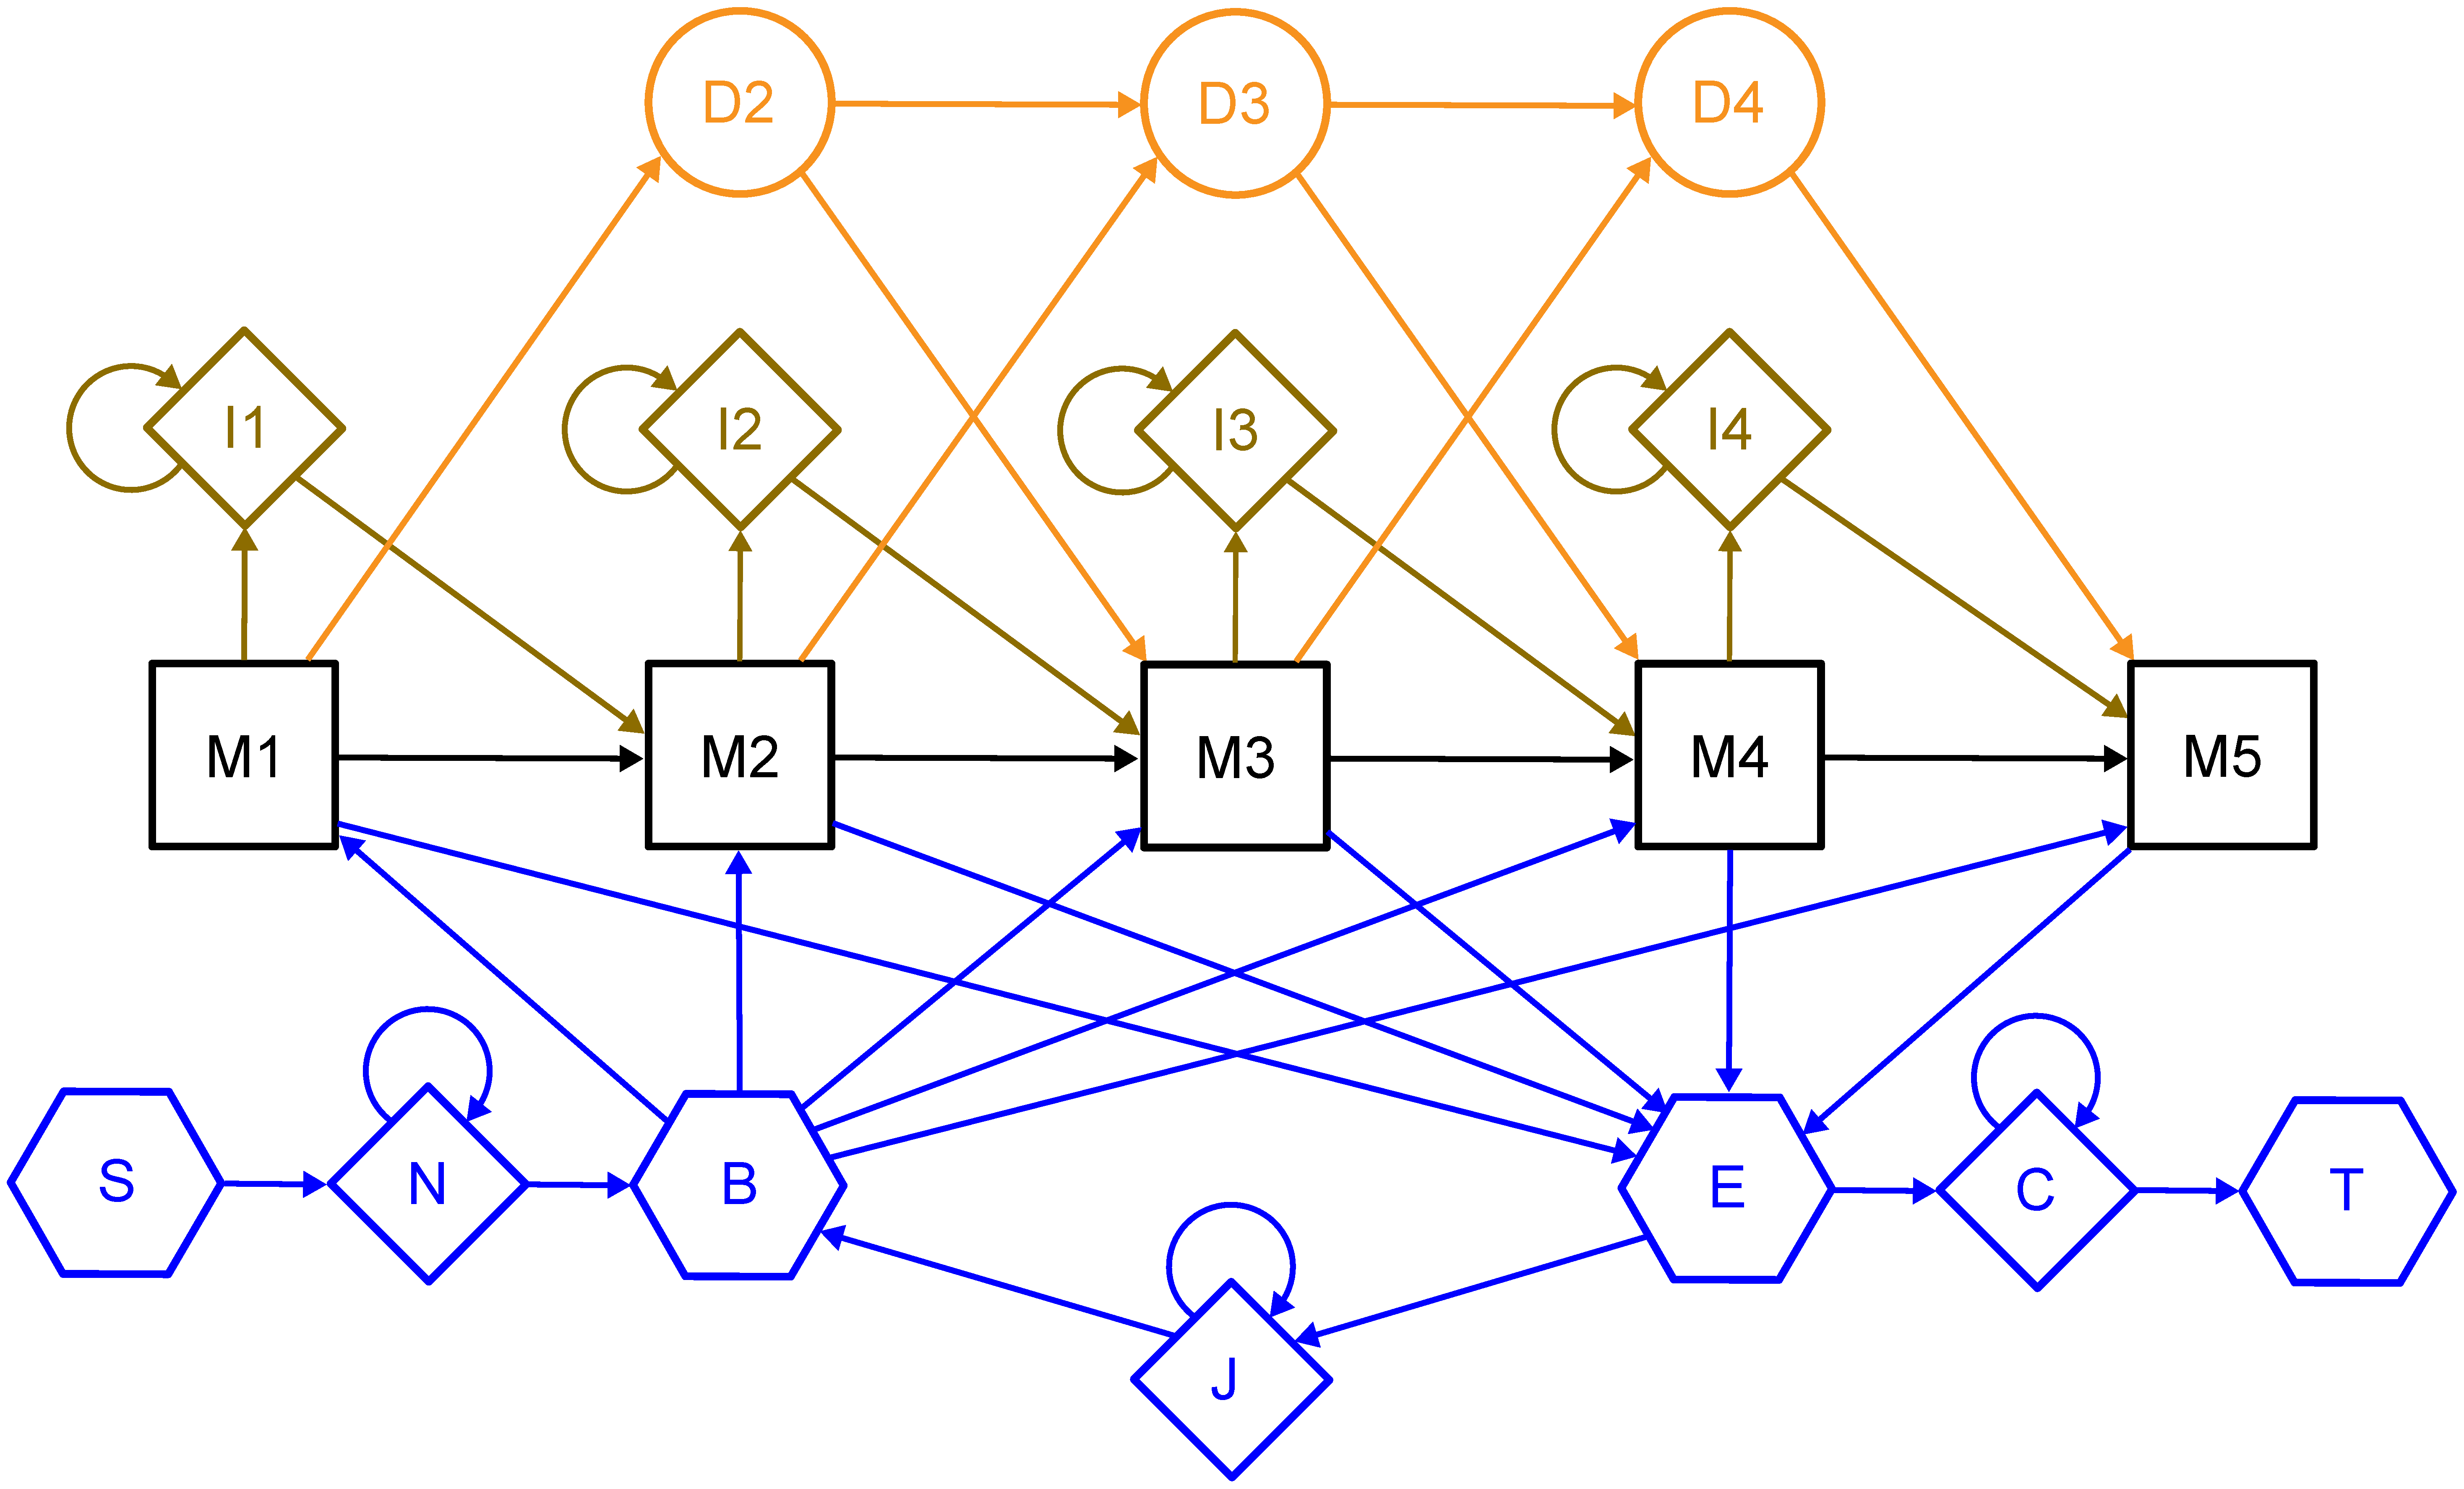
\includegraphics{img-hmm/hmmer-model.eps} }
    \caption[HMMER general model] {Complete model used by HMMER 3.0. Allows for multiple hits (multihit mode) in either local or global alignment mode. }
    \label{hmmer-model}
  \end{center}
\end{figure}

HMMER is a tool developed by Eddy \cite{eddy1998profile} that uses Hidden Markov Models to do sequence homology search. HMMER has become a very popular suite, and a strong focus of Profile \acp{HMM} research, with many efforts conducted to improve it and optimize it (\cite{hmmer-fpgas}, \cite{hmmer-gpus}, \cite{lindahl}, \cite{hmmer-mpi}, \cite{clawhmmer}).

The original version of HMMER relied on a model architecture similar to the Krogh-Haussler model, called 'Plan 9'(due to its nine transitions per state triplet). The current version employs the 'Plan 7' model architecture, shown in \autoref{hmmer-model}. The core of this architecture is similar to Krogh-Haussler/Plan 9, but Plan 7 has no D $\rightarrow$ I or I $\rightarrow$ D transitions, thus reducing the number of transitions to 7. Plus, Insert states have emission probabilities identical to the background distribution, canceling its component in the algorithm. 

Some special-states were also added to Plan 7 to allow for arbitrary restarts (thus making it a local alignment) and repeats (multihit alignment). These special states are parametrized to control the desired form of alignment (the HMMER \emph{alignment mode}). HMMER generally supports 6 different combinations of \emph{alignment modes}, formed by combining 2 options: unihit vs multihit alignments, and the basic alignment mode (global, glocal, and local). These are explained bellow: 

\begin{itemize}

\item Local mode: Aligns regions of the sequence against regions of the model. In unihit local alignment (HMMER's \emph{UNILOCAL}), only one region is matched. In multihit local alignment (HMMER's \emph{LOCAL}), multiple regions in the sequence and model are matched, and the same model region may be aligned multiple times (thus differing from classical Smith-Waterman);

\item Global mode: Aligns the whole sequence against the entire model. It corresponds to the Needleman-Wunsch algorithm. The special states self-looping states $N$, and $C$ are disabled, as well as the $B \rightarrow Mi's$ and $Mi's \rightarrow E$ transitions;

\item Glocal mode: The whole model is aligned against a subsequence of the target. This is an interesting particular alignment mode offered by HMMER. To make it work, the $B \rightarrow Mi's$ and $Mi's \rightarrow E$ transitions are disabled (thus forcing the whole alignment of the model) but the $N$ and $C$ self-looping states are enabled, to consume arbitrarily long  leading and trailing regions of the target sequence.

\end{itemize}

The original striped implementation of the Viterbi and Forward algorithms in HMMER used SSE units with 4 channels of (32 bit) floats. Floating-point values are the most suitable to the task, since we are dealing with probabilities with possibly many decimal places.

To increase the overall speedup, the data units were later changed to 8 channels of signed integer words (16 bit), through a discretization process of the floating-point probabilities. The discretization is done by a simple scaling operation, plus to an offset to gain a slightly larger representation space.

The SSE arithmetic uses signed saturation, which automatically limits overflowed values, that can then be checked for high-scoring hits. Underflows would be a problem however, since the algorithms use $-\infty$ scores as nullifying limit values, which should never touch the normal valid scores (i.e. scores without $-\infty$ terms). As such, HMMER uses a discretization range that ensures the normal scores will never underflow for model and sequence lengths below $10^{16}$ (\cite{hmmer3}).

The latest HMMER versions are HMMER 3.0, released in March 2010 \cite{hmmer3}, and HMMER 3.1b1 released recently in May 2013. 
Since HMMER 3.0, only the Local mode is supported in full; and, in particular, in the optimized implementations of the SSE-vectorized search filters. According to the author (\cite{hmmer-userguide}), accurate statistics are only available for the Local mode, and the other modes are poorly understood in terms of probabilistic significance. Furthermore, only the Local mode does not underflow the limited-precision presentation used in the SSE implementations.


\myparagraph{HMMER Pipeline}
\label{hmmer-pipeline}

HMMER 3.0 introduced a processing pipeline which uses a combination of incremental filters, each more accurate, restrictive and expensive than the previous one. \autoref{figure-hmmer-pipeline1} gives a representation of the filtering steps of the pipeline.

\begin{figure}[h!]
	\centering
	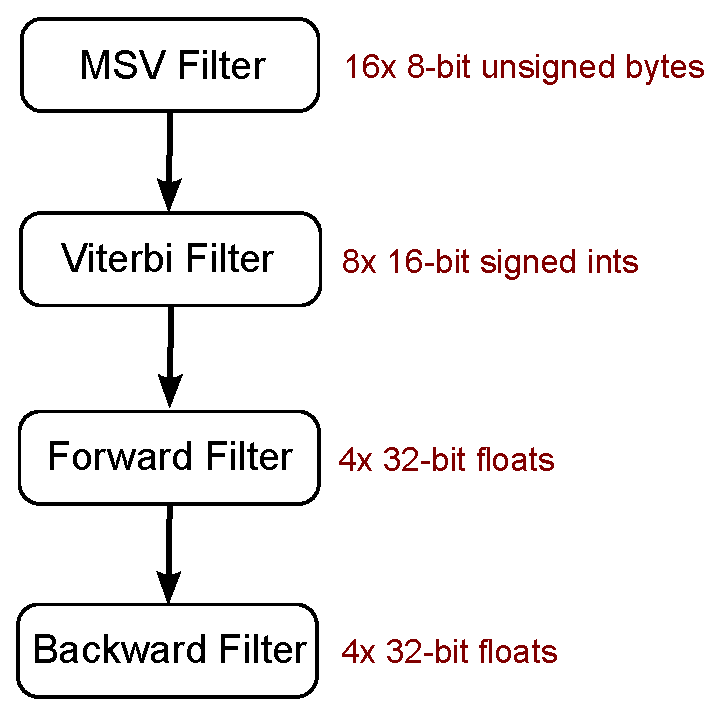
\includegraphics[scale=0.5]{img-hmm/hmmer-pipeline.eps}
	\caption{Diagram of HMMER's vectorized pipeline.}
	\label{figure-hmmer-pipeline1}
\end{figure}

The MSV (\emph{multiple segment Viterbi}) filter computes an optimal sum of multiple ungapped local alignment fragments. All of these filters have been parallelized with SSE, following Farrar's striped strategy, with increasingly higher precision. The fastest and coarser MSV filter uses 8-bit score values, the Viterbi Filter uses 16-bit scores, and the Forward and Backward filters use the full 32-bit floating point scores. In the case of Viterbi, an 8-bit precision was found to be insufficient and produce unacceptable high errors. The overall pipeline has also been parallelized to run on a multi-threaded, multi-node MPI environment with each thread processing each sequence independently.



%HMMER provides various different analysis tools, such as \emph{jackhammer} which performs an iterative database search, rebuilding and refining of the model after aligning each sequence to it, and \emph{hmmscan} which searches a target sequence against a database of profile models. On this work, the focus will be on \emph{hmmsearch}, the most used tool, that searches a target model against a sequence database.

%The application developed in this work, COPS, uses only Viterbi algorithm filter in unihit local mode (i.e., the mode more related to the original Smith-Waterman). 


%\cleardoublepage
\clearpage



